\subsection{Fourth Experience}

\subsubsection{TCP Basics}

The sequence number used to initiate the connection in the SYN segment is 0.

I have to clue where the SYN segment is.

The SYN ACK segment sent by gaia.cs.umass.edu has a sequence number of 0 as
well.

\begin{figure}[htbp]
    \centering
    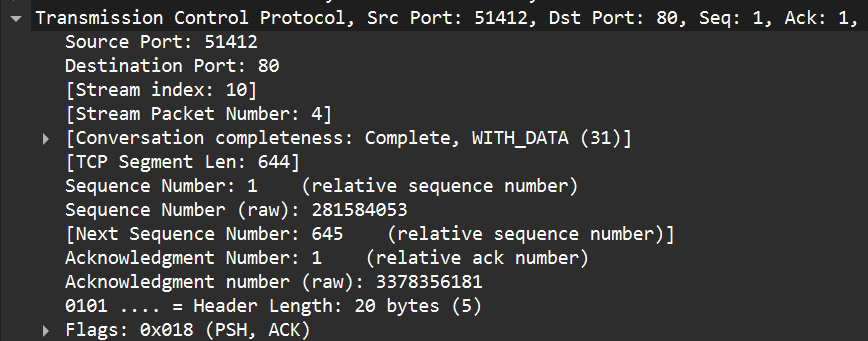
\includegraphics[width=1\linewidth]{img/fourth_experience/1.png}
    \caption{}\label{fig:4_1}
\end{figure}

The TCP segment corresponding to the POST command has two kinds of sequence
number:

\begin{itemize}
    \item Relative Seq Num: 1
    \item Raw Seq Num: 281584053
\end{itemize}

(here we say what each one means)

If we consider the POST segment to be the first one if the TCP connection, the
first six segments's data would be:

\begin{table}[htbp]
    \centering
    \begin{tabular}{|c|c|c|c|c|}
        \hline
        Segment & Sent            & ACK             & RTT        & Est. RTT     \\
        \hline
        1       & 20:34:29.490478 & 20:34:29.641190 & 0:0:150712 & 0:0:150712   \\
        2       & 20:32:29.490574 & 20:34:29.641190 & 0:0:150616 & 0:0:1507005  \\
        3       & 20:34:29.641199 & 20:34:29.688695 & 0:0:47496  & 0:0:13779994 \\
        4       & 20:34:29.786521 & 20:34:30.001886 & 0:0:215365 & 0:0:14749558 \\
        \hline
    \end{tabular}
    \caption{First six TCP segments and their sequence numbers}
    \label{tab:tcp_segments}
    % TODO: rewrite all this but pretty
\end{table}

\subsubsection{TCP Congestion Control}
% TODO: info paca